\section{Logaritmi}

\subsection{Definizione}

\begin{definition}{Logaritmo}{logaritmo}
    Dati due numeri reali positivi $a$ e $b$, con $b \neq 1$, il \textbf{logaritmo} in base $b$ di $a$ è l'esponente $c$ a cui elevare $b$ per ottenere $a$. \\[1em]
    In notazione:
    $$ \log_b(a) = c \iff b^c = a $$
    Dove:
    \begin{itemize}
        \item $b$ è la \textbf{base} ($b > 0, b \neq 1$)
        \item $a$ è l' \textbf{argomento} ($a > 0$)
        \item $c$ è il \textbf{logaritmo}
    \end{itemize}
\end{definition}

Ad esempio, $\log_2(8) = 3$ poiché $2^3 = 8$.

\subsection{Proprietà}

\begin{theorem}{Proprietà dei Logaritmi}{log_properties}
    Siano $x, y > 0$, $b > 0$ e $b \neq 1$, e $k \in \mathbb{R}$. Valgono le seguenti proprietà:
    \begin{itemize}
        \item \textbf{Logaritmo di un prodotto}: $\log_b(x \cdot y) = \log_b(x) + \log_b(y)$
        \item \textbf{Logaritmo di un quoziente}: $\log_b\left(\frac{x}{y}\right) = \log_b(x) - \log_b(y)$
        \item \textbf{Logaritmo di una potenza}: $\log_b(x^k) = k \cdot \log_b(x)$
        \item \textbf{Formula del cambio di base}: $\log_a(x) = \frac{\log_b(x)}{\log_b(a)}$
    \end{itemize}
    Inoltre, valgono questi casi notevoli:
    \begin{itemize}
        \item $\log_b(1) = 0$
        \item $\log_b(b) = 1$
    \end{itemize}
\end{theorem}

\subsection{Grafici della Funzione Logaritmica}
Il grafico della funzione $f(x) = \log_b(x)$ dipende dalla base $b$.
\begin{itemize}
    \item \textbf{Se $b > 1$}, la funzione è crescente.
    \item \textbf{Se $0 < b < 1$}, la funzione è decrescente.
\end{itemize}
In entrambi i casi, il dominio è $(0, +\infty)$ e l'asse $y$ è un asintoto verticale.

\begin{figure}[!htbp]
\centering
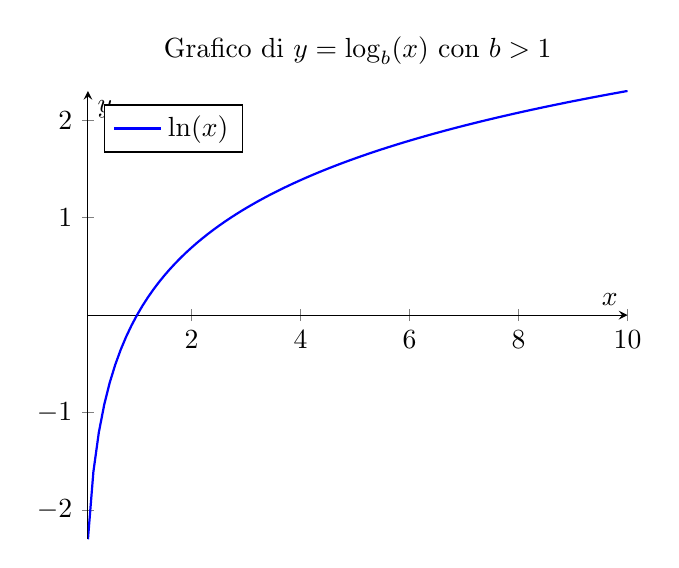
\begin{tikzpicture}
\begin{axis}[
    axis lines=middle,
    xlabel=$x$,
    ylabel=$y$,
    title={Grafico di $y = \log_b(x)$ con $b>1$},
    domain=0.1:10,
    samples=100,
    legend pos=north west
]
\addplot[blue, thick] {ln(x)};
\legend{$\ln(x)$}
\end{axis}
\end{tikzpicture}
\caption{Esempio di funzione logaritmica con base $b=e > 1$.}
\end{figure}

\begin{figure}[!htbp]
\centering
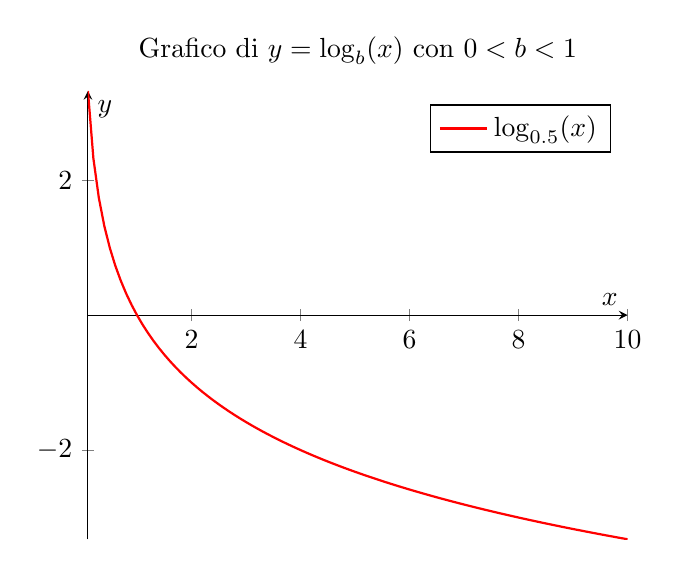
\begin{tikzpicture}
\begin{axis}[
    axis lines=middle,
    xlabel=$x$,
    ylabel=$y$,
    title={Grafico di $y = \log_b(x)$ con $0<b<1$},
    domain=0.1:10,
    samples=100,
    legend pos=north east
]
\addplot[red, thick] {log2(x)/log2(0.5)};
\legend{$\log_{0.5}(x)$}
\end{axis}
\end{tikzpicture}
\caption{Esempio di funzione logaritmica con base $b=0.5 < 1$.}
\end{figure}